\section{Linear Regression}\label{sec:linear-regression}
\framecard{\insertsection}
\subsection{Curve Fitting}

\begin{frame}{\insertsubsection}

\visible<1->{If we have a set of points in the space that comes from observations of an experiment and we want to predict other points, this could be done with \textbf{\textcolor{UniGold}{ curve fitting }}.}

\vspace{0.5em}

\visible<2->{So we could define some strategy to find our model.}

\visible<3->{
	\begin{block}{Strategy}
	\begin{itemize}
		\item[1] Purpose a \textbf{model}, e.g. functions like exponential, polynomial and others.
		\item[2] Train our model with the training data set, finding the \textbf{unknown parameters}.
	\end{itemize}
	\end{block}
}

\end{frame}


\begin{frame}{\insertsubsection}

Let's fit the points below by polynomial curve fitting

	\begin{figure}
	\label{fig:plot-fitting-example}
		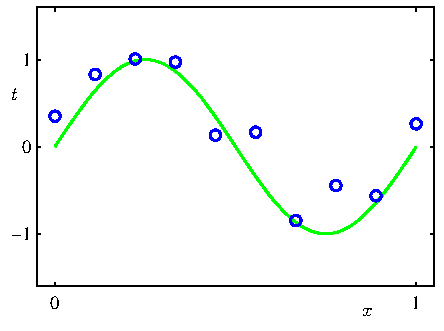
\includegraphics[totalheight=0.75\textheight]{Figure1c2.pdf}
	\end{figure}


\end{frame}

\begin{frame}{\insertsubsection}
Be the model chosen 
\visible<2->{
	\begin{align*}
		y(x,\mathbf{w}) &= w_0x^0 + w_1x^1 + w_2x^2  + ... + w_{M-1}x^{M-1}  = \sum^{M-1}_{j=1} w_j x^j
	\end{align*}
}
\visible<3->{For general, we could write this \textit{weighted sum} with any other function. In other words, we can put this in terms of $\phi_n(x)=x^n$, where $\phi$ could be other \textit{basis function}.
For simplicity, we'll carry this notation along.
}
\visible<4->{
\begin{align*}
	y(x,\mathbf{w}) &= w_0 \phi_0(x) +w_1 \phi_1(x) +w_2 \phi_2(x)  + ... + w_{M-1} \phi_{M-1}(x) = \sum^{M-1}_{j=1} w_j \phi_j(x)
\end{align*}
}
\end{frame}

\begin{frame}{\insertsubsection}

\begin{columns}
\begin{column}{0.45\textwidth}
	\visible<1->{The chosen model will give us some curve that is needed to adjust such that we'll \textit{minimize} his \textbf{distance} to the given points, or \textbf{targets} ($t$).}
	\vspace{0.5em}

	\visible<2->{Here, let's define the sum of these distances as \textit{cost function}, or loss function, and write as}

	\visible<3->{\begin{align*}
	E(\mathbf{w}) \triangleq \frac{1}{2} \sum_{n=1}^N \left\{ y_n -  t_n \right\}^2
	\end{align*}}
\end{column}
\begin{column}{0.475\textwidth}  
    \begin{center}
	\centering
	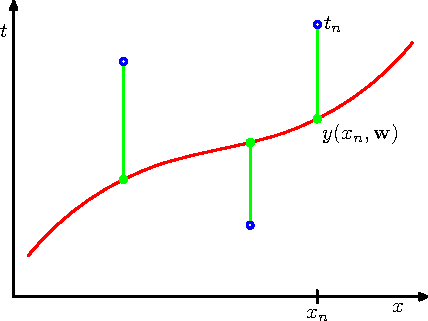
\includegraphics[totalheight=0.55\textheight]{Figure1c3.pdf}
     \end{center}
\end{column}
\end{columns}

\end{frame}
%%%%%%%%%%%%%%%%%%%%%%%%%%%%%%%%%%%
%\begin{frame}{\insertsubsection}

%\textcolor{red}{Insert some \textit{Minkowski} loss.}

%\end{frame}
%%%%%%%%%%%%%%%%%%%%%%%%%%%%%%%%
\begin{frame}{\insertsubsection}
\visible<2->{Remembering that
\begin{align*}
	y_n(x_n,\mathbf{w}) &= w_0 \phi_0(x_n) +w_1 \phi_1(x_n) +w_2 \phi_2(x_n)  + ... + w_{M-1} \phi_{M-1}(x_n)
\end{align*}
%
We could put $y_n(x_i,\mathbf{w})$ in the matricial form and get
%
\begin{equation*}
y_n
=
\begin{bmatrix}
\phi_0(x_n) & \phi_1(x_n) & ... & \phi_{M-1}(x_n)
\end{bmatrix}
\begin{bmatrix}
w_0 \\ w_1 \\  \vdots \\ w_{M-1}
\end{bmatrix}
\end{equation*}}
\end{frame}

\begin{frame}{\insertsubsection}
%
and then
%
\begin{equation*}
\underbrace{
\begin{bmatrix}
y_1 \\ y_2 \\  \vdots \\ y_N
\end{bmatrix}
}_\mathbf{y} = 
\underbrace{
\begin{bmatrix}
\phi_0(x_0) & \phi_1(x_0) & ... & \phi_{M-1}(x_0)   \\ 
\phi_0(x_1) & \phi_1(x_1) & ... & \phi_{M-1}(x_1)    \\ 
\vdots & \vdots & \ddots & \vdots \\
\phi_0(x_{N-1}) & \phi_1(x_{N-1}) & ... & \phi_{M-1}(x_{N-1})  
\end{bmatrix}
}_\Phi
\underbrace{
\begin{bmatrix}
w_1 \\ w_2 \\  \vdots \\ w_N
\end{bmatrix}
}_\mathbf{w}
\end{equation*}
This represents the system $\mathbf{y} = \Phi \mathbf{w}$. If
\begin{align*}
E(\mathbf{w}) =& \frac{1}{2} \left( \mathbf{y} - \mathbf{t} \right)^T\left( \mathbf{y} - \mathbf{t} \right)
\end{align*}
where $\mathbf{t} =
\begin{bmatrix}
t_1 & t_2 & ... & t_n
\end{bmatrix}^T
$
\end{frame}

\begin{frame}{\insertsubsection}
%
Then we'll have 
%
\begin{align*}
E(\mathbf{w}) =& \frac{1}{2} \left( \mathbf{y}^T\mathbf{y} -  \mathbf{t}^T\mathbf{y} - \mathbf{y}^T\mathbf{t} + \mathbf{t}^T\mathbf{t} \right) \\
		   =& \frac{1}{2} \left( ( \Phi \mathbf{w})^T( \Phi \mathbf{w}) -  \mathbf{t}^T( \Phi \mathbf{w}) - ( \Phi \mathbf{w})^T\mathbf{t} + \mathbf{t}^T\mathbf{t} \right) \\
		   =& \frac{1}{2} \left( \mathbf{w}^T \Phi^T \Phi \mathbf{w} -  2\mathbf{t}^T \Phi \mathbf{w} + \mathbf{t}^T\mathbf{t} \right)
\end{align*}
this by the fact that $\alpha =  \mathbf{t}^T( \Phi \mathbf{w}) = ( \Phi \mathbf{w})^T\mathbf{t}$, being $\alpha$ a scalar.

\end{frame}

\begin{frame}{\insertsubsection}
In sequence, we'll try to minimize it in terms of the weights ($\mathbf{w}$) by

\begin{align*}
	0 =& \frac{\partial E(\mathbf{w})}{\partial \mathbf{w}} \\
	0 =& \frac{1}{2} \left( 2 \mathbf{w}^T \Phi^T \Phi  -  2\mathbf{t}^T \Phi + 0 \right) \\
	\mathbf{w}^T =&  \mathbf{t}^T \Phi \left( \Phi^T \Phi \right)^{-1} \\
	\mathbf{w} =& \left( \Phi^T \Phi \right)^{-1}\Phi^T \mathbf{t} \\
\end{align*}

Here, we've obtained $\mathbf{w}$ for the curve fitting.

\end{frame}

\begin{frame}{\insertsubsection}

\begin{figure}
\begin{subfigure}{.3\textwidth}
  \centering
  \includegraphics[width=1\linewidth]{"linear_regression_M1".eps}
\end{subfigure}%
\begin{subfigure}{.3\textwidth}
  \centering
  \includegraphics[width=1\linewidth]{"linear_regression_M2".eps}
\end{subfigure}
\begin{subfigure}{.3\textwidth}
  \centering
  \includegraphics[width=1\linewidth]{"linear_regression_M5".eps}
\end{subfigure}
\begin{subfigure}{.3\textwidth}
  \centering
  \includegraphics[width=1\linewidth]{"linear_regression_M10".eps}
\end{subfigure}%
\begin{subfigure}{.3\textwidth}
  \centering
  \includegraphics[width=1\linewidth]{"linear_regression_M50".eps}
\end{subfigure}
\begin{subfigure}{.3\textwidth}
  \centering
  \includegraphics[width=1\linewidth]{"linear_regression_M100".eps}
\end{subfigure}
\end{figure}

\end{frame}

\begin{frame}{\insertsubsection}

\begin{columns}
\begin{column}{0.45\textwidth}
	\visible<1->{A visible effect of the \textit{increase of the complexity} of the model, represented here by $M$, is the \textit{increase of the weights}. We call it \textbf{over-fitting}.}
	
	\vspace{1em}
	\visible<2->{This phenomenon illustrate a method of ever search for the \textit{best estimation for the parameters}.}
	
	\vspace{1em}
	\visible<3->{It's reasonable to see that our model start's to differ from the $y$ and starts to interpolate the noise.}

	
\end{column}
\begin{column}{0.475\textwidth}  %%<--- here
    \begin{center}
	\centering
	\includegraphics[width=1\linewidth]{"linear_regression_M50".eps}
     \end{center}
\end{column}
\end{columns}

\end{frame}

\begin{frame}{\insertsubsection}

\visible<1->{ To control the over-fitting, we try to \textit{regularize} the weights by adding a penalty term ($\lambda$) to error function, by this we force the coefficients to not reach high values.}

\visible<2->{
		\begin{align*}
			\tilde{E}(\mathbf{w}) =&\frac{1}{2} (\mathbf{y}-\mathbf{t})^T(\mathbf{y}-\mathbf{t}) +\frac{\lambda}{2} \mathbf{w}^T\mathbf{w} \\
		   				    =& \frac{1}{2} \left( \mathbf{w}^T \Phi^T \Phi \mathbf{w} -  2\mathbf{t}^T \Phi \mathbf{w} + \mathbf{t}^T\mathbf{t} + \lambda \mathbf{w}^T\mathbf{I}\mathbf{w} \right) \\
	\Rightarrow \frac{\partial E(\mathbf{w})}{\partial \mathbf{w}} =& \frac{1}{2} \left( 2 \mathbf{w}^T \Phi^T \Phi  -  2\mathbf{t}^T \Phi + 0 + 2 \lambda \mathbf{w}^T \mathbf{I} \right) \\
			0 =&  \mathbf{w}^T \Phi^T \Phi  -  \mathbf{t}^T \Phi + \lambda \mathbf{w}^T \mathbf{I} \\
             \mathbf{w} = & \left( \Phi^T \Phi + \lambda \mathbf{I} \right)^{-1} \Phi^T \mathbf{t}
\end{align*}
}

\end{frame}


%%%%%%%%%%%%%%%%%%%%%%%%%%%%%%%%%%%%%%%%%%%%%%%%%
%
\subsection{A probabilistic perspective}
% \begin{frame}{\insertsubsection}
% 	\begin{tikzpicture}[thick]

% 		% Define nodes
% 		\node[latent]                               (t) 
% 			[label=north east:$t_n$] {};
% 		\node[latent, right=of t,draw=red!80, thick] (w) 
% 			[label=north east:$\mathbf{w}$]{};
	
% 		% Connect the nodes
% 		\edge [draw=red!80] {w} {t} ; %
	
% 		% Plates
% 		\plate [draw=blue!80, inner sep=10pt] {} {(t)} {$N$} ;
	
% 	\end{tikzpicture}	
% \end{frame}

\begin{frame}{\insertsubsection}
\begin{columns}
\begin{column}{0.45\textwidth}
	\visible<2->{So, we'll start to look the regression with a statistical approach. To encourage you, let's take the sentence.}
	\visible<3->{\vspace{1.5em}
		\begin{block}{Sentence}
		\textit{Having an \textbf{\textcolor{red}{uncertainty}} in the measured value, we could represent it with a  \textbf{\textcolor{red}{probability distribuition}}}.
		\end{block}
   		     }
\end{column}
\begin{column}{0.475\textwidth}  %%<--- here
    \begin{center}
		\visible<4->{
		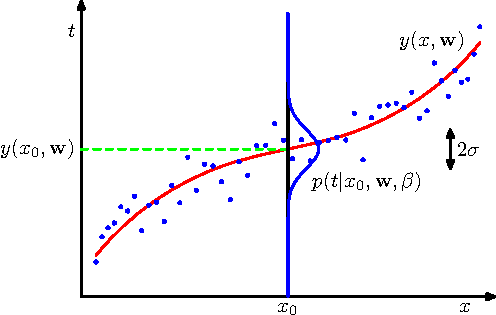
\includegraphics[totalheight=0.5\textheight]{Figure1c16.pdf}
		}
     \end{center}
\end{column}
\end{columns}
\end{frame}

\begin{frame}{\insertsubsection}
\begin{columns}
\begin{column}{0.45\textwidth}
	\visible<1->{Let's go back to the initial problem of curve fitting. Each observation of the phenomenon is described with a random variable whose \textit{mean} is given by $y(x,\mathbf{w})$, and the \textit{variance} by $\beta$. }
	\visible<2->{\vspace{1.5em}\\
			Then, we want to obtain the probability of the \textit{targets}, given some parameters, in this case $\mathbf{x}$, $\mathbf{w}$ and $\beta$.}
\end{column}
\begin{column}{0.475\textwidth}  %%<--- here
    \begin{center}
		\visible<1->{
		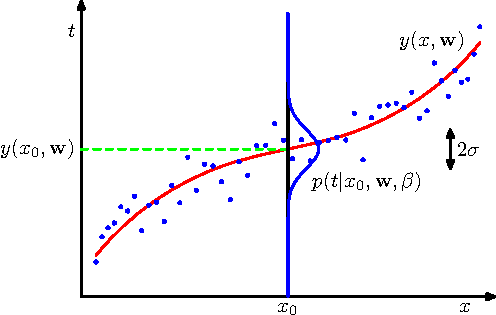
\includegraphics[totalheight=0.5\textheight]{Figure1c16.pdf}
		}
     \end{center}
\end{column}
\end{columns}
\end{frame}

\begin{frame}{\insertsubsection}	
	\visible<1->{So, if we consider that our conditions are such that being the random variables independent and identically distributed, we can say that our \textit{joint probability} is given by
	\begin{equation*}
		p(\mathbf{t} | \mathbf{x}, \mathbf{w}, \beta) = \prod_{n=1}^N p \left( t_n | x_n, \mathbf{w}, \beta \right)
	\end{equation*}
	}
	\visible<2->{Let's assume we have a distribution such that $p( \mathbf{t}| \mathbf{x}, \mathbf{w}, \beta)$. Our goal is, given the \textit{parameters}, maximize the \textit{probability} of the \textit{targets} given the \textit{parameters}. An approach to do this use the fact that
	}
	\visible<2->{
	\begin{equation*}
	\int_\infty ^{-\infty} p(x) dx = 1 \text{ and } p(x) \geq 0
	\end{equation*}}
\end{frame}

\begin{frame}{\insertsubsection}

	Seen this, we're supposing that $p$ could assume values much smaller than one. To avoid computational singularity and for future purposes, we'll take the logarithmic probability. And then
	\begin{equation*}
		\ln \left( p( \mathbf{t}| \mathbf{x}, \mathbf{w}, \beta) \right)
	\end{equation*}
	Reminding that
	\begin{equation*}
		p(\mathbf{t} | \mathbf{x}, \mathbf{w}, \beta) = \prod_{n=1}^N p \left( t_n | x_n, \mathbf{w}, \beta \right)
	\end{equation*}
	Implies that
	\begin{equation*}
		\ln \left( p( \mathbf{t}| \mathbf{x}, \mathbf{w}, \beta) \right) = \sum_{n=1}^N \ln \left(   p \left( t_n | x_n, \mathbf{w}, \beta \right) \right)
	\end{equation*}
\end{frame}

\begin{frame}{\insertsubsection}

\begin{columns}
\begin{column}{0.45\textwidth}
	\visible<1->{To proceed, we need to know what distribution $p$ is. Let's choose the \textbf{\textcolor{UniGold}{Gaussian distribution}}. \\ }
\end{column}
\begin{column}{0.475\textwidth}  %%<--- here
    \begin{center}
		\visible<1->{
		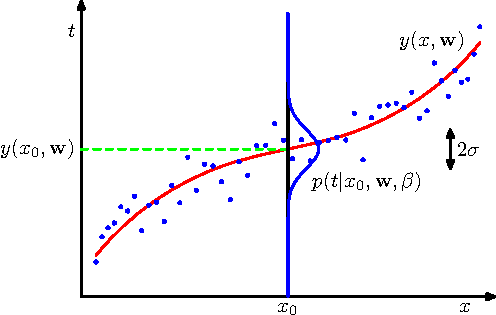
\includegraphics[totalheight=0.5\textheight]{Figure1c16.pdf}
		}
     \end{center}
\end{column}
\end{columns}
\end{frame}

\begin{frame}{\insertsubsection}
\begin{columns}
\begin{column}{0.45\textwidth}

	\visible<1->{The \textbf{\textcolor{UniGold}{Gaussian distribution}} comes from many different contexts, as the one that maximize the entropy among of all ones with fixed variance and from the sum of multiple random variables with finite variance. \\ }
	
\end{column}
\begin{column}{0.475\textwidth}  %%<--- here
    \begin{center}
		\visible<1->{
		\includegraphics[width=1\linewidth]{"Figure1.13".pdf}
		}
     \end{center}
\end{column}
\end{columns}
\end{frame}

\begin{frame}{\insertsubsection}

\begin{block}{One-dimensional Gaussian distribution}
\begin{equation*}
	\mathcal{N}(x | \mu, \sigma^2) = \frac{1}{(2 \pi \sigma^2)^{1/2}} \exp \left\{ -\frac{1}{2 \sigma^2} (x- \mu)^2 \right\} > 0
\end{equation*}
where $\mu$ is the mean and $\sigma^2$ the variance.
\end{block}

\end{frame}

\begin{frame}{\insertsubsection}

Now, back to the discussion of the maximization of 
\begin{equation*}
		\ln \left( p( \mathbf{t}| \mathbf{x}, \mathbf{w}, \beta) \right) = \sum_{n=1}^N \ln \left(   p \left( t_n | x_n, \mathbf{w}, \beta \right) \right)
\end{equation*}

\visible<2->{Reminding that
\begin{equation*}
\mathcal{N}(x | \mu, \sigma^2) = \frac{1}{(2 \pi \sigma^2)^{1/2}} \exp \left\{ -\frac{1}{2 \sigma^2} (x- \mu)^2 \right\}
\end{equation*}
we can state a Gaussian distribution for each target and then
}
\visible<3->{
\begin{equation*}
 p( t| \mathbf{x}, \mathbf{w}, \beta) = \mathcal{N} \left( t | y(\mathbf{x}, \mathbf{w}), \beta^{-1} \right)
\end{equation*}
}

\end{frame}

\begin{frame}{\insertsubsection}
\visible<1->{
And then, from the \textit{joint probability} of the Gaussians distributions

\begin{equation*}
		\ln \left( p( \mathbf{t}| \mathbf{x}, \mathbf{w}, \beta) \right) = \sum_{n=1}^N - \frac{1}{2} \ln (2 \pi) + \sum_{n=1}^N \frac{1}{2} \ln \beta - \sum_{n=1}^N \frac{\beta}{2} (x_n -  y(x_n, \mathbf{w}))^2
\end{equation*}
}
\visible<2->{From this, we could obtain the \textbf{maximum likelihood}, or the \textit{best estimation for the parameters}, taking the derivatives of the log probability to zero, according to the terms $\beta$ and $\mathbf{w}$, our model parameters. We'll obtain
\begin{equation*}
\frac{1}{\beta_{ML}} = \frac{1}{N} \sum^N_{n=1} \left\{ y(x_n, \mathbf{w}_{ML}) - t_n \right\}^2
\end{equation*}
remembering that $\mathbf{w}_{ML}$ is already known from the regular linear regression.
}
%Maximizing with respect to $\beta$, we'll have 

%\begin{equation*}
%		\frac{1}{\beta_{ML}} = \frac{1}{N} \sum^N_{n=1} \left\{ y(x_n, \mathbf{w}_{ML}) - t_n \right\}^2
%\end{equation*}
%
%where $\beta_{ML}$ is the precision parameter for the maximum likelihood for the conditional Gaussian distribution.
\end{frame}

\begin{frame}{\insertsubsection}
We could observe that taking the derivative with respect to $\mathbf{w}$, our expression becomes closer to the \textit{error function} presented previously, added the dependency of $\beta$

\begin{align*}
	E(\mathbf{w}) \triangleq \frac{1}{2} \sum_{n=1}^N \left\{ y_n -  t_n \right\}^2
\end{align*}

Then some behaviors could be expected, as the \textbf{over-fitting}.

%Maximizing with respect to $\beta$, we'll have 

%\begin{equation*}
%		\frac{1}{\beta_{ML}} = \frac{1}{N} \sum^N_{n=1} \left\{ y(x_n, \mathbf{w}_{ML}) - t_n \right\}^2
%\end{equation*}
%
%where $\beta_{ML}$ is the precision parameter for the maximum likelihood for the conditional Gaussian distribution.
\end{frame}

\begin{frame}{\insertsubsection}

At this point, we have a probabilistic model and we may want to predict values for $x$. Then, we need a \textit{predictive distribution}. \\
\vspace{1em}
Let's say we have the probabilities of some idea we desire to update it in the light of some new evidence. This could be done with \textbf{Bayes' Theorem}, to convert a \textit{prior} probability in a \textit{posterior} probability. \\
\end{frame}

\begin{frame}{\insertsubsection}
Mathematically, by Bayes' Theorem and the \textbf{Product Rule}, we could infer
\visible<2->{
\begin{equation*}
p\left( \mathbf{w} | \mathbf{x}, \mathbf{t}, \alpha, \beta \right) \propto p\left(  \mathbf{t} |\mathbf{w} ,\mathbf{x}, \beta \right)  p\left( \mathbf{w} | \alpha \right)
\end{equation*}
}
\visible<3->{
and for simplicity, consider the follow prior for $\mathbf{w}$
\begin{equation*}
p \left( \mathbf{w} | \alpha \right) = \mathcal{N} \left( \mathbf{w} | \boldsymbol{0}, \alpha^{-1} \mathbf{I} \right) = \left(  \frac{\alpha}{2 \pi}\right) ^{(M+1)/2} \exp \left\{ - \frac{\alpha}{2} \mathbf{w}^T \mathbf{w} \right\}
\end{equation*}
where $\alpha$ the precision of the distribution and $M+1$ is the dimension of $\mathbf{w}$, for a polynomial of $M^{th}$ order. Variables such $\alpha$ are called \textit{hyperparameters} and control the distribuition of model parameters.}
\end{frame}

\begin{frame}{\insertsubsection}
By this, we can find a distribution and its maximum, or most probable value of $\mathbf{w}$ given the data taking the minimum of the negative logarithm of the infered expression, that will lead us to a term

\begin{equation*}
\sum^N_{n=1} \left\{ y(x_n, \mathbf{w}) - t_n \right\}^2 + \frac{\alpha}{2} \mathbf{w}^T\mathbf{w} + \text{const.}
\end{equation*}

Note that if we consider $\lambda = \alpha / \beta$, this will back to the regularized form of \textit{least squares}.
\end{frame}

\begin{frame}{\insertsubsection}

So, observe that even making some probabilistic assumptions, we don't have yet a fully bayesian model, given that finding the \textit{maximum likelihood}, we're finding only the parameters given one model such that maximize our targets probabilities. Furthermore, even with some probabilistic assumptions, our model still have a \textbf{over-fitting} problem, given that we obtained the same expressions for the simple regression, adding some constants.\\
\vspace{1em}
The next step is put some \textbf{uncertainty in predictive model}, and makes adjustments in the light of our new evidences. By that we could obtain a "more Bayesian" model, in other words, a \textcolor{UniGold}{\textbf{Bayesian Linear Regression}}.

\end{frame}

%\begin{frame}{\insertsubsection}
%	\visible<1->{Let's take a look at the Bayes Theorem}
%	
%	\visible<2->{
%	\begin{block}{Bayes Theorem}{
%			\begin{equation*}\label{bayes_theorem}
%				\visible<2->{ p(\mathbf{w}|\mathcal{D}) = \frac{p(\mathcal{D}| \mathbf{w}) p(\mathbf{w}) } {  p(\mathcal{D}) } } 
%			\end{equation*}
%			}
%	\end{block}
%	\visible<3->{The new role of Bayes Theorem here is the fact that we could obtain new, or better, probability distribuitions for the weights in light of an determined data set $\mathcal{D}$.}
%	}
%\end{frame}

%\begin{frame}{\insertsubsection}
%	\visible<1->{\textbf{\textcolor{UniGold}{At this time, it's important to point out some things. \\}}}
%	\vspace{1.5em}
%	\visible<2->{When we write $ p \left( t_n | x_n, \mathbf{w}, \beta \right)$, we assume a probability distribuition over the parameters $\mathbf{w}$ and $\beta$ too.\\}
%	\vspace{1.5em}
%	\visible<3->{Then we could observe that we'll obtain a \textbf{discrete distribution of functions} in their \textit{parameters}.\\}
%	\vspace{1.5em}
%	\visible<4->{So, here is where the Bayes Theorem plays an important role by \textbf{adjusting} these \textit{parameters} as we obtain evidences.}
%\end{frame}
%
%\begin{frame}{\insertsubsection}
%	\visible<1->{Taking some steps back, let's re-visit the \textbf{Curve Fitting}. There, the strategy was minimize the error function.\vspace{1.5em} \\}
%	\visible<2->{Now we'll try to view the same problem with a \textit{probabilistic perspective}. We're trying to make predictions for the target value $\mathbf{t}$ given some new values of $x$.\vspace{1.5em} \\}
%
%\end{frame}


%\begin{frame}{\insertsubsection}
%	And taking the derivatives with respect to $\beta$ to minimize the error	
%		\begin{align*}
%		\visible<1->{
%			\frac{\partial}{\partial \beta}\ln \left( p( \mathbf{t}| \mathbf{x}, \mathbf{w}, \beta) \right) &=0 } \\
%		\visible<2->{
%			 -\frac{1}{2} \sum^N_{n=1} \left\{ y(x_n,\mathbf{w} -t_n ) \right\}^2 + \frac{N}{2}\frac{1}{\beta} &= 0 \\  }
%		\visible<3->{
%			 \frac{1}{N} \sum^N_{n=1} \left\{ y(x_n,\mathbf{w} -t_n ) \right\}^2  &= \frac{1}{\beta_{ML}}  }
%		\end{align*}
%	\visible<4->{
%	Where $\beta_{ML}$ is the maximum likelihood.}
%
%\end{frame}